\renewcommand*{\arraystretch}{1.1}

\subsection*{Interactive / complex / 11}
\label{section:interactive-complex-read-11}

% change \emph{} to use sans-serif font
\let\oldemph\emph
\renewcommand{\emph}[1]{{\footnotesize \sf #1}}

\renewcommand{\currentQueryCard}{11}
\marginpar{
	\raggedleft
	\vspace{0.22ex}

	\queryRefCard{interactive-complex-read-01}{Interactive}{1}\\
	\queryRefCard{interactive-complex-read-02}{Interactive}{2}\\
	\queryRefCard{interactive-complex-read-03}{Interactive}{3}\\
	\queryRefCard{interactive-complex-read-04}{Interactive}{4}\\
	\queryRefCard{interactive-complex-read-05}{Interactive}{5}\\
	\queryRefCard{interactive-complex-read-06}{Interactive}{6}\\
	\queryRefCard{interactive-complex-read-07}{Interactive}{7}\\
	\queryRefCard{interactive-complex-read-08}{Interactive}{8}\\
	\queryRefCard{interactive-complex-read-09}{Interactive}{9}\\
	\queryRefCard{interactive-complex-read-10}{Interactive}{10}\\
	\queryRefCard{interactive-complex-read-11}{Interactive}{11}\\
	\queryRefCard{interactive-complex-read-12}{Interactive}{12}\\
	\queryRefCard{interactive-complex-read-13}{Interactive}{13}\\
	\queryRefCard{interactive-complex-read-14}{Interactive}{14}\\
}

\noindent\begin{tabularx}{\queryCardWidth}{|>{\queryPropertyCell}p{\queryPropertyCellWidth}|X|}
	\hline
	query & Interactive / complex / 11 \\ \hline
%
	title & Job referral \\ \hline
%
	pattern & \hfill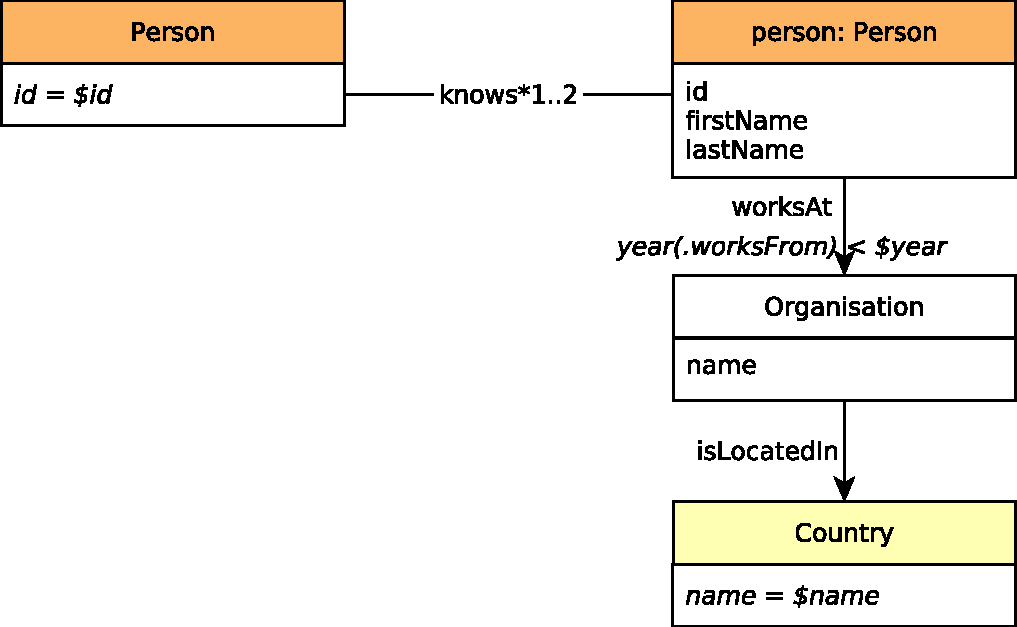
\includegraphics[scale=\patternscale,margin=0cm .2cm]{patterns/interactive-complex-read-11}\hfill \\ \hline
%
	desc. & Given a start Person, find that Person's friends and friends of friends
(excluding start Person) who started Working in some Company in a given
Country, before a given date (year).
 \\ \hline
%
	
		params &
		\innerCardVSpace{\begin{tabularx}{\attributeCardWidth}{|>{\paramNumberCell}c|>{\varNameCell}M|>{\typeCell}m{\typeWidth}|Y|} \hline
		$\mathsf{1}$ & Person.id
 & ID
 &  \\ \hline
		$\mathsf{2}$ & Country.name
 & String
 &  \\ \hline
		$\mathsf{3}$ & year
 & 32-bit Integer
 &  \\ \hline
		\end{tabularx}}\innerCardVSpace \\ \hline
	
%
	
		result &
		\innerCardVSpace{\begin{tabularx}{\attributeCardWidth}{|>{\resultNumberCell}c|>{\varNameCell}M|>{\typeCell}m{\typeWidth}|>{\resultOriginCell}c|Y|} \hline
		$\mathsf{1}$ & Person.id & ID & R &
				 \\ \hline
		$\mathsf{2}$ & Person.firstName & String & R &
				 \\ \hline
		$\mathsf{3}$ & Person.lastName & String & R &
				 \\ \hline
		$\mathsf{4}$ & Person-worksAt-\textgreater{}Organisation.name & String & R &
				 \\ \hline
		$\mathsf{5}$ & Person-worksAt-\textgreater{}.worksFrom & 32-bit Integer & R &
				 \\ \hline
		\end{tabularx}}\innerCardVSpace \\ \hline
	
%
	
		sort		&
		\innerCardVSpace{\begin{tabularx}{\attributeCardWidth}{|>{\sortNumberCell}c|>{\varNameCell}M|>{\directionCell}c|Y|} \hline
		$\mathsf{1}$ & Person-worksAt-\textgreater{}.worksFrom
 & $\asc
$ &  \\ \hline
		$\mathsf{2}$ & Person.id
 & $\asc
$ &  \\ \hline
		$\mathsf{3}$ & Person-worksAt-\textgreater{}Organisation.name
 & $\desc
$ &  \\ \hline
		\end{tabularx}}\innerCardVSpace \\ \hline
	%
	limit & 10 \\ \hline
	%
	CPs &
	\multicolumn{1}{>{\raggedright}l|}{
		\chokePoint{1.4}, 
		\chokePoint{2.3}, 
		\chokePoint{2.4}, 
		\chokePoint{3.3}
		} \\ \hline
	%
	relevance &
		\small This query looks for paths of length two or three, starting from a Person, moving to friends or friends of friends,
and ending at a Company. In this query, there are selective joins and a top k order by that can be exploited for
optimizations.
 \\ \hline%
\end{tabularx}
\queryCardVSpace

% change \emph back to the old one
\renewcommand{\emph}[1]{\oldemph{#1}}